\chapter{Representing Graphs}
\label{ch:graphs}

\newcommand{\lecnum}{23}
%\newcommand{\lectitle}{Representing Graphs}
\newcommand{\lecturer}{Frank Pfenning, Andr\'e Platzer, Rob Simmons,\\
  Penny Anderson, Iliano Cervesato}

\chapterTAGS{application, complexity, graph, graph-representation, interface}
\maketitle

\begin{preamble}
\noindent
In this lecture we introduce \emph{graphs}.  Graphs provide a uniform
model for many structures, for example, maps with distances or
Facebook relationships.  Algorithms on graphs are therefore important
to many applications.  They will be a central subject in the
algorithms courses later in the curriculum; here we only provide a
very basic foundation for graph algorithms.
\end{preamble}

\begin{gram}[Learning Goals]
With respect to our learning goals we will look at the following
notions.
\begin{description}
\item[Computational Thinking: ]%
  We get a taste of the use of graphs in computer science.  We note that some
  graphs are represented explicitly while others are kept implicit.
\item[Algorithms and Data Structures: ]%
  We see two basic ways to represent graphs: using adjacency matrices and by
  means of adjacency lists.
\item[Programming: ]%
  We use linked lists to give an adjacency list implementation of graphs.
\end{description}
\end{gram}

\clearpage
\section{Undirected Graphs}
\label{sec:graphs:undirected_graphs}
\TAGS{application, graph}

We start with \emph{undirected graphs} which consist of a set $V$ of
\emph{vertices} (also called \emph{nodes}) and a set $E$ of
\emph{edges}, each connecting two different vertices.  The following
is a simple example of an undirected graph with 5 vertices ($A, B, C,
D, E$) and 6 edges ($AB$, $BC$, $CD$, $AE$, $BE$, $CE$):
\begin{center}
  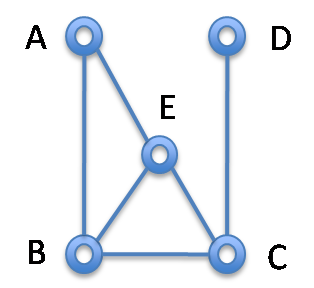
\includegraphics[width=0.3\textwidth]{img/graph0.png}
\end{center}

We don't distinguish between the edge $AB$ and the edge $BA$ because
we're treating graphs as undirected.  There are many ways of defining
graphs with slight variations. Because we specified above that each
edge connects two different vertices, no vertex in a graph can have an
edge from a node back to itself in this course.


\section{Implicit Graphs}
\label{sec:graphs:implicit_graphs}
\TAGS{application, graph}

There are many, many different ways to represent graphs.  In some
applications they are never explicitly constructed but remain implicit
in the way the problem was solved. The game of \emph{Lights Out} is one
example of a situation that implicitly describes an undirected graph.
Lights Out is an electronic game consisting of a grid of lights,
usually 5 by 5. The lights are initially pressed in some pattern of on
and off, and the objective of the game is to turn all the lights off.
The player interacts with the game by touching a light, which toggles
its state and the state of all its cardinally adjacent neighbors (up,
down, left, right).
\begin{center}
  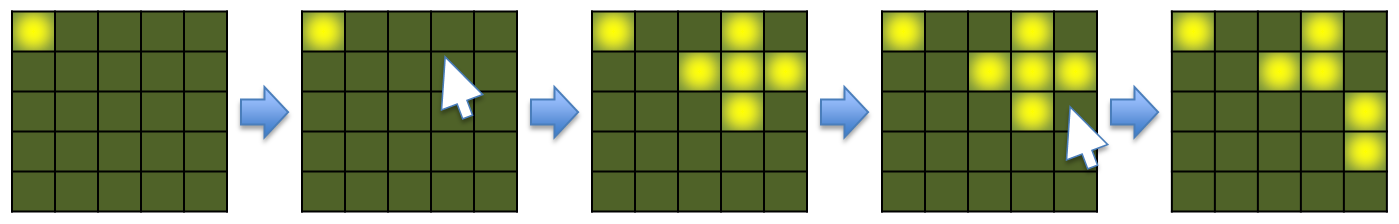
\includegraphics[width=0.9\textwidth]{img/lightsout.png}
\end{center}
We can think of lights out as an implicit graph with $2^{25}$ vertices, one
for every possible configuration of the 5x5 lights out board, and an edge
between two vertices if we can transition from one board to another with a
single button press.  If we transition from one board to another by pressing a
button, we can return to the first board by pressing the \emph{same} button.
Therefore the graph is undirected.
\begin{center}
  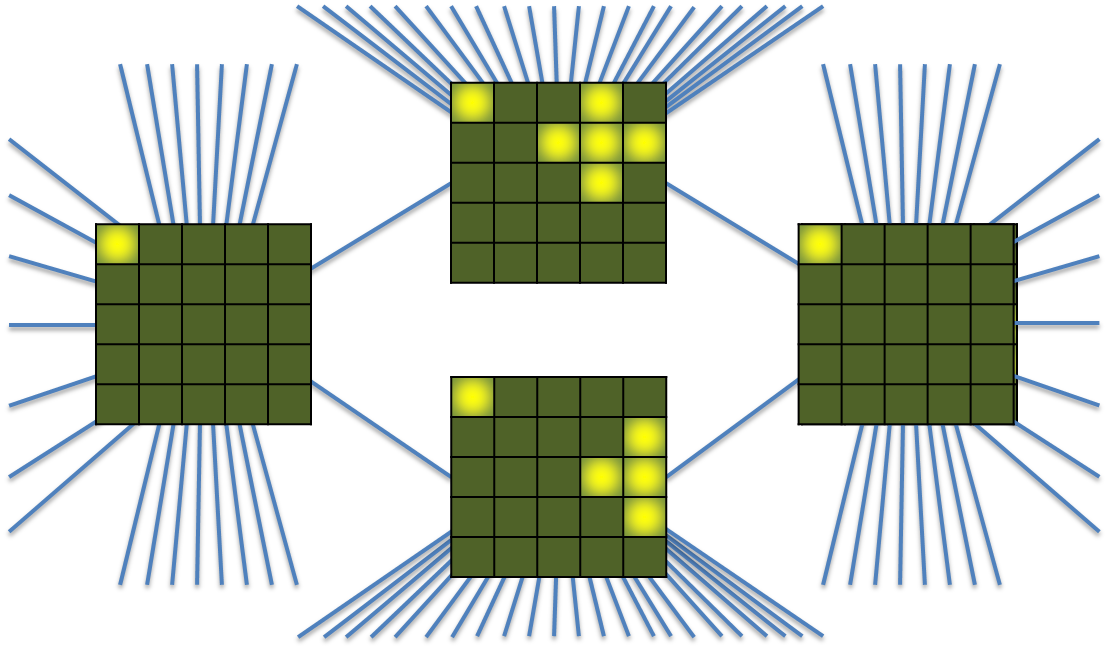
\includegraphics[width=0.55\textwidth]{img/lightsout-graph.png}
\end{center}
Each of the $2^{25}$ vertices is therefore connected to 25 different edges,
giving us $25 \times 2^{25} / 2$ total edges in this graph --- we divide by 2
because going to a node and coming back from it are expressed by the same
edge. But because the graph is implicit in the description of the Lights Out
game, we don't have to actually store all ~32 million vertices and ~400
million edges in memory to understand Lights Out.

An advantage to thinking about Lights Out as a graph is that we can
think about the game in terms of graph algorithms.  Asking whether
we can get all the lights out for a given board is asking whether the vertex
representing our starting board is connected to the board with all the
lights out by a series of edges: a \emph{path}. We'll talk more about
this \emph{graph reachability} question in the next lecture.


\section{Explicit Graphs and a Graph Interface}
\label{sec:graphs:graph_interface}
\TAGS{graph, interface}

Sometimes we \emph{do} want to represent a graph as an explicit set of
edges and vertices and in that case we need a graph datatype. In the C
code that follows, we'll refer to our vertices with unsigned integers.
The minimal interface for graphs in Figure~\ref{fig:graphs:graph_h} allows us
to create and free graphs, check whether an edge exists in the graph,
add a new edge to the graph, and get and free a list of the neighbors
of a node.

\begin{gram}[graph.h]
\label{fig:graphs:graph_h}
\begin{figure}[h!]
\begin{lstlisting}[language=c, aboveskip=0pt, belowskip=0pt]
typedef unsigned int vertex;
typedef struct graph_header *graph_t;

graph_t graph_new(unsigned int numvert);
//@ensures \result != NULL;

void graph_free(graph_t G);
//@requires G != NULL;

unsigned int graph_size(graph_t G);
//@requires G != NULL;

bool graph_hasedge(graph_t G, vertex v, vertex w);
//@requires G != NULL;
//@requires v < graph_size(G) && w < graph_size(G);

void graph_addedge(graph_t G, vertex v, vertex w);
//@requires G != NULL;
//@requires v < graph_size(G) && w < graph_size(G);
//@requires v != w && !graph_hasedge(G, v, w);

typedef struct vert_list_node vert_list;
struct vert_list_node {
  vertex vert;
  vert_list *next;
};

vert_list* graph_get_neighbors(graph_t G, vertex v);
//@requires G != NULL;
//@requires v < graph_size(G);

void graph_free_neighbors(vert_list* neighbors);
\end{lstlisting}
\caption{A simple graph interface --- \lstinline'graph.h'}
\end{figure}
\end{gram}

We use the C0 notation for contracts on the interface functions here.
Even though C compilers do not recognize the \requires{}
contract and will simply discard it as a comment, the contract still
serves an important role for the programmer reading the program.  For
the graph interface, we decide that it does not make sense to add an
edge into a graph when that edge is already there, hence the second
precondition.  A neighbor list is just a linked list of nodes.

With this minimal interface, we can create a graph for what will be
our running example (letting A = 0, B = 1, and so on):

\noindent
\begin{minipage}{0.6\textwidth}
\begin{lstlisting}[language=c]
  graph_t G = graph_new(5);
  graph_addedge(G, 0, 1); // AB
  graph_addedge(G, 1, 2); // BC
  graph_addedge(G, 2, 3); // CD
  graph_addedge(G, 0, 4); // AE
  graph_addedge(G, 1, 4); // BE
  graph_addedge(G, 2, 4); // CE
\end{lstlisting}
\end{minipage}%
\begin{minipage}{0.4\textwidth}
\begin{center}
  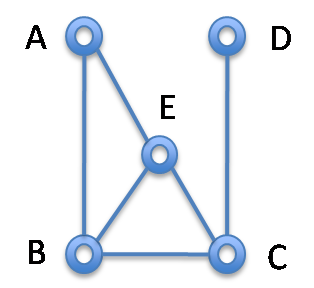
\includegraphics[width=0.6\textwidth]{img/graph0.png}
\end{center}
\end{minipage}

We could implement the graph interface in Figure~\ref{fig:graphs:graph_h} in
a number of ways. In the simplest form, a graph with $e$ edges can be
represented as a linked list or array of edges. In the linked list
implementation, it takes $O(1)$ time to add an edge to the graph with
\lstinline'graph_addedge', because it can be appended to the front of
the linked list. Finding whether an edge exists in a graph with $e$
edges might require traversing the whole linked list, so
\lstinline'graph_hasedge' is an $O(e)$ operation.  Getting the
neighbors of a node would take $O(e)$.

Hashtables and balanced binary search trees would be our standard
tools in this class for representing sets of edges more
efficiently. Instead of taking that route, we will discuss two classic
structures for directly representing graphs.


\section{Adjacency Matrices}
\label{sec:graphs:adjmatrix}
\TAGS{complexity, graph-representation}

One simple way is to represent the graph as a two-dimensional array that
describes its edge relation as follows.
\begin{center}
  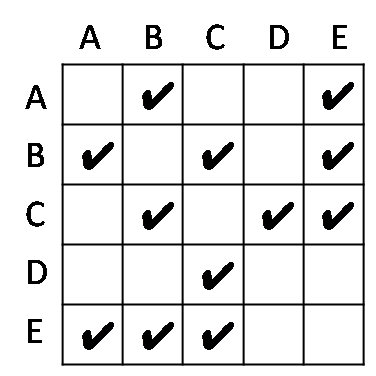
\includegraphics[width=0.38\textwidth]{img/adj-matrix0.png}
\end{center}
There is a checkmark in the cell at row $v$ and column $v'$ exactly when there
is an edge between nodes $v$ and $v'$.  This representation of a graph is
called an \emph{adjacency matrix}, because it is a matrix that stores which
nodes are neighbors.

We can check if there is an edge from B (= 1) to D (= 3) by looking
for a checkmark in row 1, column 3. In an undirected graph, the
top-right half of this two-dimensional array will be a mirror image of
the bottom-left, because the edge relation is symmetric.  Because we
disallowed edges between a node and itself, there are no checkmarks on
the main diagonal of this matrix.

The adjacency matrix representation requires a lot of space: for a graph
with $v$ vertices we must allocate space in $O(v^2)$. However, the
benefit of the adjacency matrix representation is that adding an edge
(\lstinline'graph_addedge') and checking for the existence of an edge
(\lstinline'graph_hasedge') are both $O(1)$ operations.

Are the space requirements for adjacency matrices (requires space in
$O(v^2)$) worse than the space requirements for storing all the edges
in a linked list (requires space in $O(e)$)? That depends on the
relationship between $v$, the number of vertices, and $e$ the number
of edges. A graph with $v$ vertices has between 0 and ${v\choose 2} =
\frac{v(v-1)}{2}$ edges. If most of the edges exist, so that the
number of edges is proportional to $v^2$, we say the graph is
\emph{dense}. For a dense graph, $O(e) = O(v^2)$, and so adjacency
matrices are a good representation strategy for dense graphs, because
in big-$O$ terms they don't take up more space than storing all the
edges in a linked list, and operations are much faster.


\section{Adjacency Lists}
\label{sec:graphs:adjlist}
\TAGS{complexity, graph-representation}

If a graph is not dense, then we say the graph is \emph{sparse}. The other
classic representation of a graphs, \emph{adjacency lists}, can be a good
representation of sparse graphs.

In an adjacency list representation, we have a
one-dimensional array that looks much like a hash table. Each vertex
has a spot in the array, and each spot in the array contains a linked
list of all the other vertices connected to that vertex. Our running
example would look like this as an adjacency list:
\begin{center}
  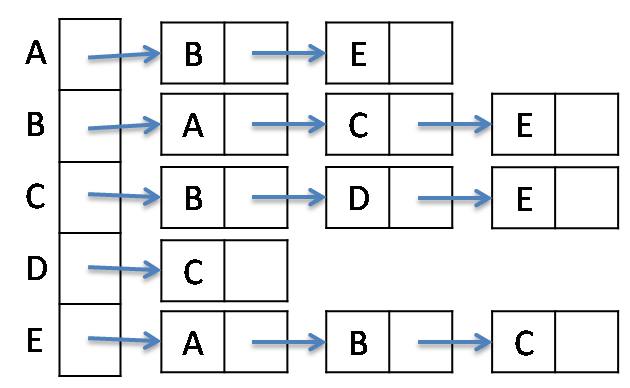
\includegraphics[width=0.6\textwidth]{img/adj-list.png}
\end{center}

Adjacency lists require $O(v+e)$ space to represent a graph with $v$
vertices and $e$ edges: we have to allocate a single array of length
$v$ and then allocate two list entries per edge.  The complexity class
$O(v+e)$ is often written as $O(\max(v,e))$ --- we leave it as an
exercise to check that these two classes are equivalent --- and
therefore this is the notation we will typically use.  Adding an edge
is still constant time, but lookup (\lstinline'graph_hasedge') now
takes time in $O(\min(v,e))$, since $\min(v-1,e)$ is the maximum
length of any single adjacency list.  Finding the neighbors of a node
is immediate with an adjacency list representation as we simply return
the adjacency list of that node --- this has cost $O(1)$.  This is in
contrast with the adjacency matrix representation where we are forced
to check every value on the row of the matrix corresponding to that
node.

\bigskip%
The following table summarizes and compares the asymptotic cost
associated with the adjacency matrix and adjacency list
implementations of a graph, under the assumptions used in this
chapter.
$$
\renewcommand{\arraystretch}{1.5}
\begin{array}{|l|c|c|}
\hline
  & \textbf{Adjacency Matrix} & \textbf{Adjacency List}
\\\hline\hline
  \text{Space}                   & O(v^2)       & O(\max(v,e))
\\\hline
  \mathtt{graph\_hasedge}        & O(1)         & O(\min(v,e))
\\\hline
  \mathtt{graph\_addedge}        & O(1)         & O(1)
\\\hline
  \mathtt{graph\_get\_neighbors} & O(v)         & O(1)
\\\hline
\end{array}
$$
The cost of \lstinline'graph_hasedge' can be reduced by storing the
neighbors of each node not in a linked list but in a more
search-efficient data structure, for example an AVL tree or a hash
set.  Of course, doing so requires additional space, something that
may not be desirable in some applications.  It also comes at the
expense of \lstinline'graph_get_neighbors'.


\section{Adjacency List Implementation}
\label{sec:graphs:adjlist_impl}
\TAGS{graph-representation}

The header for a graph is a struct with two fields: the first is an
unsigned integer representing the actual size, and the second is an
array of adjacency lists.  We use the vertex list from the graph
interface as our adjacency list.
\begin{lstlisting}[language=c]
typedef vert_list adjlist;

typedef struct graph_header graph;
struct graph_header {
  unsigned int size;
  adjlist **adj;
};
\end{lstlisting}

\noindent
We leave it as an exercise to the reader to define the representation functions
\begin{lstlisting}[language=c]
bool is_vertex(graph *G, vertex v)
bool is_graph(graph *G)
\end{lstlisting}
that check that a vertex is valid for a given graph and that a graph
itself is valid.

We can allocate the struct for a new graph using \lstinline'xmalloc',
since we're going to have to initialize both its fields anyway. But
we'd definitely allocate the adjacency list itself using
\lstinline'xcalloc' to make sure that it is initialized to array full
of \lstinline'NULL' values: empty adjacency lists.
\begin{lstlisting}[language=c]
graph *graph_new(unsigned int size) {
  graph *G = xmalloc(sizeof(graph));
  G->size = size;
  G->adj = xcalloc(size, sizeof(adjlist*));
  ENSURES(is_graph(G));
  return G;
}
\end{lstlisting}

Given two vertices, we have to search through the whole adjacency list
of one vertex to see if it contains the other vertex. This is what
gives the operation a running time in $O(\min(v,e))$.
\begin{lstlisting}[language=c]
bool graph_hasedge(graph *G, vertex v, vertex w) {
  REQUIRES(is_graph(G) && is_vertex(G, v) && is_vertex(G, w));

  for (adjlist *L = G->adj[v]; L != NULL; L = L->next) {
    if (L->vert == w) return true;
  }
  return false;
}
\end{lstlisting}

Because we assume an edge must not already exist when we add it to the
graph, we can add an edge in constant time:
\begin{lstlisting}[language=c]
void graph_addedge(graph *G, vertex v, vertex w) {
  REQUIRES(is_graph(G) && is_vertex(G, v) && is_vertex(G, w));
  REQUIRES(v != w && !graph_hasedge(G, v, w));

  adjlist *L;

  L = xmalloc(sizeof(adjlist));  // add w as a neighbor of v
  L->vert = w;
  L->next = G->adj[v];
  G->adj[v] = L;

  L = xmalloc(sizeof(adjlist));  // add v as a neighbor of w
  L->vert = v;
  L->next = G->adj[w];
  G->adj[w] = L;

  ENSURES(is_graph(G));
  ENSURES(graph_hasedge(G, v, w));
}
\end{lstlisting}

Finding the neighbors of a vertex is just a matter of returning its
adjacency list.
\begin{lstlisting}[language=c]
vert_list *graph_get_neighbors(graph *G, vertex v) {
  REQUIRES(is_graph(G) && is_vertex(G, v));
  return G->adj[v];
}
\end{lstlisting}

It is tempting to implement the operation
\lstinline'graph_free_neighbors' so that it frees every node in its
input neighbor list.  But this would destroy our representation since
\lstinline'graph_get_neighbors' returned an \emph{alias} into the adjacency
list representation of the graph.  Instead, we shall define this
function so that it does nothing
\begin{lstlisting}[language=c]
void graph_free_neighbors(vert_list *L) {
  (void)L;
}
\end{lstlisting}
Here, \lstinline'(void)L' serves the purpose of fooling the compiler
into believing that this function is using the variable
\lstinline'L'.  Without it, our standard compilation flags would cause
it to report an error.


\section{Iterating through a Graph}
\label{sec:graphs:print_edges}
\TAGS{complexity, graph-representation}

To gain practice with working with our graph interface, we write a
function that prints all the edges in a graph.  Give it a try and then
check your work on the next page.  This function has the following
prototype:
\begin{lstlisting}[language=c]
void graph_print(graph_t G)
\end{lstlisting}


\newpage
Our implementation is as follows:
\begin{lstlisting}[language=c]
void graph_print(graph_t G) {
  for (vertex v = 0; v < graph_size(G); v++) {
    printf("Vertices connected to %u: ", v);
    vert_list *nbors = graph_get_neighbors(G, v);
    for (vert_list *p = nbors; p != NULL; p = p->next) {
      vertex w = p->vert;   // w is a neighbor of v
      printf(" %u,", w);
    }
    graph_free_neighbors(nbors);
    printf("\n");
  }
}
\end{lstlisting}
The outer loop examines all the vertices in the graph.  For each of
them, we compute its neighbor list and then go through it in the inner
loop to print them.  We call the function
\lstinline'graph_free_neighbors' to dispose of the neighbor list once
we are done with it.  In our adjacency list representation, this
call does nothing, but this won't be the case for an adjacency
matrix representation for example.  Not calling it may cause a memory
leak depending on which implementation we use.

It is interesting to analyze the complexity of \lstinline'graph_print'
on a graph containing $v$ vertices and $e$ edges.  The outer loop runs
$v$ times.  Inside this loop, the following operations take place:
\begin{itemize}
\item%
  Some print statements that we may assume have cost $O(1)$.
\item%
  A call to \lstinline'graph_get_neighbors', whose cost is constant in
  the adjacency list representation but $O(v)$ in the adjacency matrix
  representation.  Up to this point in the code, the cost of our
  function is $O(v)$ in the former representation and $O(v^2)$ in the
  latter.
\item%
  The inner loop, whose body performs constant cost operations.  In
  isolation, the body of this loop runs $O(v)$ times since each vertex
  can have up to $v-1$ neighbors.  Thus, a naive analysis gives us an
  $O(v^2)$ worst case complexity for \lstinline'graph_print' with both
  representations up to this point in the code.

  However, each neighbor corresponds to an edge in the graph.
  Therefore, the body of the inner loop will be executed exactly $2e$
  times total over an entire run of \lstinline'graph_print' --- each
  edge is examined twice, once from each of its endpoints.  Thus the
  inner loop has cost $O(e)$ \emph{overall}.  Adding this to our
  tally, the cost of \lstinline'print_graph' to this point in our
  analysis is $O(\max(v,e))$ --- which we recall is the common way of
  writing $O(v+e)$ --- in the adjacency list representation, and
  $O(\max(v^2, e))$ for the adjacency matrix representation.  Since $e
  \in O(v^2)$ for any graph, the latter expression simplifies to
  $O(v^2)$.

\item%
  A call to \lstinline'graph_free_neighbors'.  This has constant cost
  in the adjacency list representation.  By the same reasoning we just
  performed for the inner loop, this will have cost $O(e)$
  \emph{overall} in the adjacency matrix representation.
\end{itemize}
Summarizing, our analysis tells us that \lstinline'graph_print' has
cost $O(\max(v,e))$ in the adjacency list representation and $O(v^2)$
with the adjacency matrix representation.  For a dense graph --- where $e
\in O(v^2)$ --- these two expressions are equivalent.  For a sparse
graph, the former can be significantly cheaper.


\clearpage
\section{Exercises}
\label{sec:graphs:exercises}

\begin{exercise}
  Define the representation functions \lstinline'is_graph' and
  \lstinline'is_vertex' (and any other you may need) used in the
  contracts of the adjacency matrix implementation in
  Section~\ref{sec:graphs:adjlist_impl} of the graph interface of
  Section~\ref{sec:graphs:graph_interface}.
\end{exercise}

\begin{exercise}
  Give an implementation of the graph interface in
  Section~\ref{sec:graphs:graph_interface} based on adjacency matrices.  Make
  sure to provide adequate representation functions.
\end{exercise}
